%%%%%%%%%%%%%%%%%%%%%%%%%%%%%%%%%%%%%%%
% Wenneker Resume/CV
% LaTeX Template
% Version 1.1 (19/6/2016)
%
% This template has been downloaded from:
% http://www.LaTeXTemplates.com
%
% Original author:
% Frits Wenneker (http://www.howtotex.com) with extensive modifications by 
% Vel (vel@LaTeXTemplates.com)
%
% License:
% CC BY-NC-SA 3.0 (http://creativecommons.org/licenses/by-nc-sa/3.0/
%
%%%%%%%%%%%%%%%%%%%%%%%%%%%%%%%%%%%%%%
\def\as{$^{\prime\prime}$ }
\def\asno{$^{\prime\prime}$}
\def\am{$^{\prime}$ }
\def\amno{$^{\prime}$}
\def\amp{\&}
\def\co{$^{13}$CO }
\def\cono{$^{13}$CO}
\def\hi{\textsc{Hi} }
\def\hino{\textsc{Hi}}
\def\hii{\textsc{Hii} region }
\def\hiino{\textsc{Hii} region}
\def\hiis{\textsc{Hii} regions }
\def\hiisno{\textsc{Hii} regions}
\def\jyb{Jy~beam$^{-1}$ }
\def\jybno{Jy~beam$^{-1}$}
\def\kms{km~s$^{-1}$ }
\def\kmsno{km~s$^{-1}$}
\def\mw{Milky Way }
\def\mwno{Milky Way}
\def\nh{N$_{\rm H}$ }
\def\nhno{N$_{\rm H}$}
\def\gp{Galactic Plane }
\def\gpno{Galactic Plane}
\def\gd{Galactocentric distance }
\def\gdno{Galactocentric distance}
\def\gmc{Giant Molecular Clouds }
\def\gmc{Giant Molecular Clouds}
\def\gmcs{Giant Molecular Clouds }
\def\gmcsno{Giant Molecular Clouds}
\def\td{3D }
\def\tdno{3D}

\newcommand{\aap}{A\&A}
\newcommand{\aaps}{A\&AS}
\newcommand{\mnras}{MNRAS}
\newcommand{\apj}{ApJ}
\newcommand{\pjl}{ApJL} 
\newcommand{\apjs}{ApJS} 
\newcommand{\pasj}{PASJ}
\newcommand{\aj}{AJ}
\newcommand{\araa}{ARA\&A}
\newcommand{\pasa}{PASA}
\newcommand{\aspc}{ASPC}
\newcommand{\apss}{Ap\&SS}
\newcommand{\pasp}{PASP}
\newcommand{\farcm}{\mbox{\ensuremath{.\mkern-4mu^\prime}}}%    % fractional arcminute symbol: 0.'0
\newcommand{\farcs}{\mbox{\ensuremath{.\!\!^{\prime\prime}}}}%  % fractional arcsecond symbol: 0.''0
\newcommand{\fdg}{\mbox{\ensuremath{.\!\!^\circ}}}%             % fractional degree symbol:     0.°0



%----------------------------------------------------------------------------------------
%	PACKAGES AND OTHER DOCUMENT CONFIGURATIONS
%----------------------------------------------------------------------------------------

\documentclass[a4paper,12pt]{memoir} % Font and paper size

\usepackage{natbib}

%%%%%%%%%%%%%%%%%%%%%%%%%%%%%%%%%%%%%%%%%
% Wenneker Resume/CV
% Structure Specification File
% Version 1.1 (19/6/2016)
%
% This file has been downloaded from:
% http://www.LaTeXTemplates.com
%
% Original author:
% Frits Wenneker (http://www.howtotex.com) with extensive modifications by 
% Vel (vel@latextemplates.com)
%
% License:
% CC BY-NC-SA 3.0 (http://creativecommons.org/licenses/by-nc-sa/3.0/)
%
%%%%%%%%%%%%%%%%%%%%%%%%%%%%%%%%%%%%%%%%%

%----------------------------------------------------------------------------------------
%	PACKAGES AND OTHER DOCUMENT CONFIGURATIONS
%----------------------------------------------------------------------------------------

\usepackage{XCharter} % Use the Bitstream Charter font
\usepackage[utf8]{inputenc} % Required for inputting international characters
\usepackage[T1]{fontenc} % Output font encoding for international characters

\usepackage[top=1cm,left=1cm,right=1cm,bottom=1cm]{geometry} % Modify margins

\usepackage{graphicx} % Required for figures

\usepackage{flowfram} % Required for the multi-column layout

\usepackage{url} % URLs

\usepackage[usenames,dvipsnames]{xcolor} % Required for custom colours

\usepackage{tikz} % Required for the horizontal rule

\usepackage{enumitem} % Required for modifying lists
\setlist{noitemsep,nolistsep} % Remove spacing within and around lists

\setlength{\columnsep}{\baselineskip} % Set the spacing between columns

% Define the left frame (sidebar)
\newflowframe{0.2\textwidth}{\textheight}{0pt}{0pt}[left]
\newlength{\LeftMainSep}
\setlength{\LeftMainSep}{0.2\textwidth}
\addtolength{\LeftMainSep}{1\columnsep}
 
% Small static frame for the vertical line
\newstaticframe{1.5pt}{\textheight}{\LeftMainSep}{0pt}
 
% Content of the static frame with the vertical line
\begin{staticcontents}{1}
\hfill
\tikz{\draw[loosely dotted,color=RoyalBlue,line width=1.5pt,yshift=0](0,0) -- (0,\textheight);}
\hfill\mbox{}
\end{staticcontents}
 
% Define the right frame (main body)
\addtolength{\LeftMainSep}{1.5pt}
\addtolength{\LeftMainSep}{1\columnsep}
\newflowframe{0.7\textwidth}{\textheight}{\LeftMainSep}{0pt}[main01]

\pagestyle{empty} % Disable all page numbering

\setlength{\parindent}{0pt} % Stop paragraph indentation


%----------------------------------------------------------------------------------------
%	NEW COMMANDS
%----------------------------------------------------------------------------------------

\newcommand{\userinformation}[1]{\renewcommand{\userinformation}{#1}} % Define a new command for the CV user's information that goes into the left column

\newcommand{\cvheading}[1]{{\Huge\bfseries\color{RoyalBlue} #1} \par\vspace{.6\baselineskip}} % New command for the CV heading
\newcommand{\cvsubheading}[1]{{\Large\bfseries #1} \bigbreak} % New command for the CV subheading

\newcommand{\Sep}{\vspace{1em}} % New command for the spacing between headings
\newcommand{\SmallSep}{\vspace{0.5em}} % New command for the spacing within headings

\newcommand{\aboutme}[2]{ % New command for the about me section
\textbf{\color{RoyalBlue} #1}~~#2\par\Sep
}
	
\newcommand{\CVSection}[1]{ % New command for the headings within sections
{\Large\textbf{#1}}\par
\SmallSep % Used for spacing
}

\newcommand{\CVItem}[2]{ % New command for the item descriptions
\textbf{\color{RoyalBlue} #1}\par
#2
\SmallSep % Used for spacing
}

\newcommand{\bluebullet}{\textcolor{RoyalBlue}{$\circ$}~~} % New command for the blue bullets

 % Include the file specifying document layout and packages

%----------------------------------------------------------------------------------------
%	NAME AND CONTACT INFORMATION 
%----------------------------------------------------------------------------------------

\userinformation{ % Set the content that goes into the sidebar of each page
\begin{flushright}
% Comment out this figure block if you don't want a photo
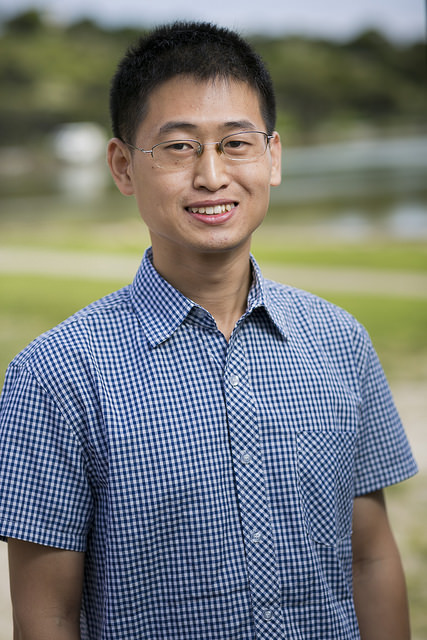
\includegraphics[width=0.6\columnwidth]{hongquan.jpg}\\[\baselineskip] % Your photo
\small % Smaller font size
Hongquan Su \\ % Your name

\tiny
\url{hongquan.su@icrar.org} \\ % Your email address
\url{hongquansu.github.io} \\ % Your URL
+61 8 9266 1289 \\ % Your phone number
\Sep % Some whitespace
\textbf{Address} \\
1 Turner Av \\ % Address 1
Perth, WA 6102 \\ % Address 2
Australia \\ % Address 3
\vfill % Whitespace under this block to push it up under the photo
\end{flushright}
}

%----------------------------------------------------------------------------------------

\begin{document}

\userinformation % Print your information in the left column

\framebreak % End of the first column

%----------------------------------------------------------------------------------------
%	HEADING
%----------------------------------------------------------------------------------------

\cvheading{Hongquan Su} % Large heading - your name

\cvsubheading{PhD candidate in radio astronomy} % Subheading - your occupation/specialization

%----------------------------------------------------------------------------------------
%	ABOUT ME
%----------------------------------------------------------------------------------------

\aboutme{About Me}{The beautiful Milky Way attracts me to explore its structure and various sources in it with two observational techniques named neutral hydrogen absorption and \hii absorption at radio frequencies.}

%----------------------------------------------------------------------------------------
%	EDUCATION
%----------------------------------------------------------------------------------------

\CVSection{Education}

%------------------------------------------------

\CVItem{2005 - 2009, Bachelor of Physics, Xuzhou Normal University}

%------------------------------------------------

\CVItem{2009 - 2012, Master of Astrophysics, Beijing Normal University}

%------------------------------------------------

\CVItem{2012 - 2014, Research assistant, National Astronomical Observatories of China}

%------------------------------------------------

\CVItem{2014 - now, PhD candidate, Curtin University}

%------------------------------------------------

\Sep % Extra whitespace after the end of a major section

%------------------------------------------------

\Sep % Extra whitespace after the end of a major section

\CVSection{Conferences}

%------------------------------------------------

\CVItem{SPARCS VII THE PRECURSORS AWAKEN}{ Oral Talk: Measuring and modeling the Galactic synchrotron emission distribution with the GLEAM survey}

%------------------------------------------------

\Sep % Extra whitespace after the end of a major section

%----------------------------------------------------------------------------------------
%	SKILLS
%----------------------------------------------------------------------------------------

\CVSection{Outreach}
\CVItem{2014}{Guild pupils to have a telescope viewing at Lakelands sky view night}

%------------------------------------------------
\CVItem{2015}{Talk about astronomy with a large variety of audience at the open day of Curtin University}

\CVItem{2016}{Introducing my work to high school students}

%------------------------------------------------

\Sep % Extra whitespace after the end of a major section

%----------------------------------------------------------------------------------------
%	NEW PAGE DELIMITER
%	Place this block wherever you would like the content of your CV to go onto the next page
%----------------------------------------------------------------------------------------



%----------------------------------------------------------------------------------------
%	AWARDS
%----------------------------------------------------------------------------------------


%------------------------------------------------

\Sep % Extra whitespace after the end of a major section

%----------------------------------------------------------------------------------------
%	INTERESTS
%----------------------------------------------------------------------------------------

\CVSection{Interests}

%------------------------------------------------

Data analysis, Python, fits file operation, MCMC fitting

\Sep
%------------------------------------------------

\Sep % Extra whitespace after the end of a major section

%----------------------------------------------------------------------------------------

\CVSection{Publications}
% use generate_publication_list to get the list

\CVItem{Journal papers}{

\textbf{Su, H.}, Hurley-Walker, N., Jackson, C. A., McClure-Griffiths, N. M., Tingay,
S. J., Hindson, L., Hancock, P., Wayth, R. B., Gaensler, B. M., Staveley-
Smith, L., Morgan, J., Johnston-Hollitt, M., Lenc, E., Bell, M. E., Calling-
ham, J. R., Dwarkanath, K. S., For, B.-Q., Kapinska, A. D., McKinley, B.,
Offringa, A. R., Procopio, P., Wu, C., and Zheng, Q. (2017a). \textit{Galactic syn-
chrotron emissivity measurements between 250 < l < 355 degrees from the
GLEAM survey with the MWA}. \textbf{MNRAS}, 465:3163–3174.
\\

\clearpage % Start a new page

\userinformation % Print your information in the left column

\framebreak % End of the first column
%---------------------------------------------------

%\textbf{Su, H.}, Hurley-Walker, N., Jackson, C. A., McClure-Griffiths, N. M., Tingay,
%S. J., Hindson, L., Hancock, P., Wayth, R. B., Gaensler, B. M., Staveley-
%Smith, L., Morgan, J., Johnston-Hollitt, M., Lenc, E., Bell, M. E., Call-
%ingham, J. R., Dwarkanath, K. S., For, B.-Q., Kapinska, A. D., McKinley,
%B., Offringa, A. R., Procopio, P., Wu, C., and Zheng, Q. (2017b). Erratum:
%Galactic synchrotron emissivity measurements between 250 < l < 355 degrees
%from the GLEAM survey with the MWA. \textbf{MNRAS}, 472:828–834.
%\\
%---------------------------------------------------

\textbf{Su, H.}, et al., \textit{Galactic synchrotron emissivity measurements in the
whole GLEAM survey area}. \textbf{MNRAS}, in prep.
\\

\textbf{Su, H.-Q.}, Zhang, M.-F., Zhu, H., and Wu, D. (2017c). \textit{The revised distance
of supernova remnant G15.4+0.1}. \textbf{Research in Astronomy and Astrophysics},
17:109. \\

%------------------------------------------------

% non-first author journal papers
Ai, M., Zhu, M., Xiao, L., and \textbf{Su, H.-Q.} (2013). \textit{Properties of the UCHII 
region G25.4NW and its associated molecular cloud}. \textbf{Research in Astronomy and Astrophysics}, 13:935-944.
\\
%------------------------------------------------

Hindson, L., Johnston-Hollitt, M., Hurley-Walker, N., Callingham, J. R., \textbf{Su, H.}, Morgan, J., Bell, M., Bernardi, G., Bowman, J. D., Briggs, F., Cappallo,
R. J., Deshpande, A. A., Dwarakanath, K. S., For, B.-Q., Gaensler, B. M., Greenhill, L. J., Hancock, P., Hazelton, B. J., Kapinska, A. D., Kaplan,
D. L., Lenc, E., Lonsdale, C. J., Mckinley, B., McWhirter, S. R., Mitchell,
D. A., Morales, M. F., Morgan, E., Oberoi, D., Offringa, A., Ord, S. M.,
Procopio, P., Prabu, T., Shankar, N. U., Srivani, K. S., Staveley-Smith, L.,
Subrahmanyan, R., Tingay, S. J., Wayth, R. B., Webster, R. L., Williams, A.,
Williams, C. L., Wu, C., and Zheng, Q. (2016). \textit{A Large-Scale, Low-Frequency
Murchison Widefield Array Survey of Galactic HII Regions between 260 $<$ l $<$ 340}. \textbf{PASA}, 33:e020.
\\
%------------------------------------------------

Zhu, H., Tian, W. W., Torres, D. F., Pedaletti, G., and \textbf{Su, H. Q.} (2013). \textit{A Kinematic Distance Study of the Planetary Nebulae-Supernova remnant-HII Region Complex at G35.6-0.5}. \textbf{ApJ}, 775:95.
\\
}




\CVItem{Conference papers}{
\textbf{Su, H.}, Li, Q.-K., Zhu, H., and Tian, W.-W. (2013). \textit{78 Pairs of Possible PSR-SNR Associations}. ArXiv e-prints. \\

%------------------------------------------------

\textbf{Su, H.}, Tian, W., Zhu, H., and Xiang, F. Y. (2014). \textit{Kinematic Distances of SNRs W44 and 3C 391}. In Ray, A. and McCray, R. A., editors, Supernova
Environmental Impacts, volume 296 of IAU Symposium, pages 372-373.\\

%------------------------------------------------

Tian, W., Leahy, D., Zhu, H., and \textbf{Su, H.} (2014a). \textit{Two GeV-TeV Supernova
Remnants without Associated Neutral and Molecular Clouds}. In Cami, J.
and Cox, N. L. J., editors, The Diffuse Interstellar Bands, volume 297 of IAU
Symposium, pages 229–231. \\

%------------------------------------------------

Tian, W. W., Leahy, D. A., and \textbf{Su, H.} (2014b). \textit{Multi-band Observation of
TeV Supernova Remnants}. In Ray, A. and McCray, R. A., editors, Supernova
Environmental Impacts, volume 296 of IAU Symposium, pages 374–375. \\

%------------------------------------------------

Tian, W.-W., \textbf{Su, H.}, and Xiang, F. Y. (2013). \textit{The Galactic NH - AV Relation
and its Application to Historical Galactic SNRs}. ArXiv e-prints. \\

%------------------------------------------------

Zhu, H., Tian, W., \textbf{Su, H.}, and Wu, D. (2014). \textit{Kinematic Distance of Galactic
Radio Objects}. In Cami, J. and Cox, N. L. J., editors, The Diffuse Interstellar
Bands, volume 297 of IAU Symposium, pages 232–234.

}



%\bibliographystyle{apalike}
%\bibliography{/home/aquan/Dropbox/references/bibtex.bib}


\end{document}
